\chapter{Volkswirtschaftliche und deskriptive Standortmodelle} % (fold)
\label{cha:volkswirtschaftliche_und_deskriptive_standortmodelle}

  \section{Volkswirtschaftliche Standortmodelle} % (fold)
  \label{sec:volkswirtschaftliche_standortmodelle}

    \subsection{Die Wahl kostenminimaler Wohnstandorte} % (fold)
    \label{sub:die_Wahl_kostenminimaler_Wohnstandorte}
    
      \par \textbf{standortbezogenen Kosten}

      \begin{equation}
        C(d) = Q\cdot p(d) + V\cdot k(d)
        \label{standortbezogenen Kosten}
      \end{equation}

      % \begin{quote}
        \begin{itemize}
          \item $d$: die Entfernung des Standortes zum Stadtzentrum
          \item $C(d)$: die gesamten Standortkosten
          \item $Q$: die vorgegebene Größe der Wohnfläche
          \item $p(d)$: die standortabhängigen Mietkosten pro Flaâcheneinheit (z.B.Quadratmeter)
          \item $V$: die Anzahl der Fahrten ins Zentrum
          \item $k(d)$: standortabhängigen Fahrtkosten
        \end{itemize}
      % \end{quote}

      \par \textbf{Annahme}

      \begin{itemize}
        \setlength{\itemsep}{1pt}
        \setlength{\parskip}{0pt}
        \setlength{\parsep}{0pt}
        \item $p(d)$ nehmen mit zunehmender Entfernung zum Stadtzentrum exponentiell ab:
          
          \begin{equation}
            p(d) = P_Z \cdot e^{-rd}
          \end{equation}

          \begin{itemize}
            \item $P_Z$: der Mietpreis direkt im Zentrum
            \item $r$: Verfallskonstante für die Entfernung
          \end{itemize}

        \item die Fahrtkosten sind proportional zur Entfernung zum Zentrum

          \begin{equation}
            k(d) = K \cdot d
          \end{equation}

          \begin{itemize}
            \item $K$: die Kosten pro Entfernungseinheit
          \end{itemize}
      \end{itemize}

      \par Den kostenminimalen Standort findet man unter diesen Annahmen durch Minimierung der Funktion $C(d)$.

      \par Ableiten der Funktion $C$ nach $d$ und anschließendem ``Nullsetzen'' der Ableitung $\Rightarrow$

      

      \begin{equation}
        d^* = \frac{1}{r}(\ln[r \cdot P_Z \cdot Q] - \ln[V \cdot K])
      \end{equation}

      \begin{exmp}
        \color{blue}{Aufgabe 1, Aufgabe 2}
      \end{exmp}
    % subsection Die Wahl kostenminimaler Wohnstandorte (end)

    \subsection{Theorie der Boden- und Flächennutzung} % (fold)
    \label{sub:theorie_der_boden_und_fla_chennutzung}

    \par \textbf{von Thünens Modell}

    \begin{itemize}
      \item das zu untersuchende Gebiet ist eine kreisförmige, isolierte Fläche gleichmäßiger
Produktivität
      \item es liegt ein einziger Absatzmarkt im Zentrum der Fläche vor
      \item die Transportverbindungen sind überall gleichmäßig gut
      \item die Produktion der Produkte ist überall und zu gleichen Kosten möglich
      \item die Transportkosten steigen proportional zur Entfernung
      \item es ist eine Menge von Produktions-Aktivitäten und deren Output-Mengen gegeben
    \end{itemize}

    \par Unter dem Gesichtspunkt der Gewinn-Maximierung stellt sich nun die Frage: 

    \textbf{``Welches der Produkte soll in welcher Entfernung vom
Absatzmarkt hergestellt werden?''}
  
    \vspace{1cm}

    \begin{algorithm}[H]
        \caption{Verfahren (zur Bestimmung der oberen Einhüllenden)}
        % \textbf{Input}: Anzahl Suchrichtungen $K, \beta, V, p$
        \begin{algorithmic}[1]
          % \Procedure{MyProcedure}{}
          \State Stelle für jede Produktions-Aktivität die zugehörige Profitfunktion auf:
          \begin{equation*}
            R(d) = \underset{i}{\text{max}}R_i(d) = \underset{i}{\text{max}}(p_i - k_id)
          \end{equation*}
          
          \State Setze $d' = 0$ und $I = {1, \dots, n}, L = \emptyset$

          \State Bestimme der max. Profit $R_{i^*} = \underset{j = 1, \dots, n}{max}R_{j}(0)$ und damit die im Zentrum profitabelste Aktivität $P_{i^*}$

          \If{(das Maximum ist nicht eindeutig)} 
            \State wähle unter den maximalen Aktivitäten diejenige mit dem kleinsten $k_j$.
          \EndIf

          \State $I = I \backslash \{i^*\}, L = L \cup \{i^* \}$

          \While{$\text{(Es gibt Schnittpunkte} (d_{ij} = \frac{P_i - P_j}{k_i - k_j}) \text{)} \wedge (I \neq \emptyset)$}
            \State Schneide $R_{i^*}$ mit allen $R_j(\cdot), j \in I$ 
            \State Bestimme $S_{i^{*}j} = (d_{i^{*}j}, R_{i^{*} \backslash j}(d_{i^{*}j})$ als den Schnittpunkt mit dem kleinsten Wert $d_{i^{i^{*}j}} > d'$
            \If{(Schneiden sich mehrere Profitfunktionen bei $d_{i^{i^{*}j}}$)}
              \State wähle unter den Aktivitäten diejenige mit dem kleinsten $k$.  
            \EndIf
            \State $d' = d_{i^{i^{*}j}}, i^{*} = j, I = I \backslash \{i^*\}$
            \State Füge $d$ und $i^*$ am Ende der Liste $L$ an
          \EndWhile

          \State Füge $d^{\text{max}}$ am Ende von $L$ ein
          
          % \EndProcedure
        \end{algorithmic}
        \textbf{Output:} Die Liste $L$ enthält dann die gesuchten Entfernungsintervalle und die zugehörigen, profitablen Produktionsaktivitäten.
      \end{algorithm}

      \newpage

      \begin{exmp}

      \end{exmp}

        \begin{figure}[htbp]
          \centering
          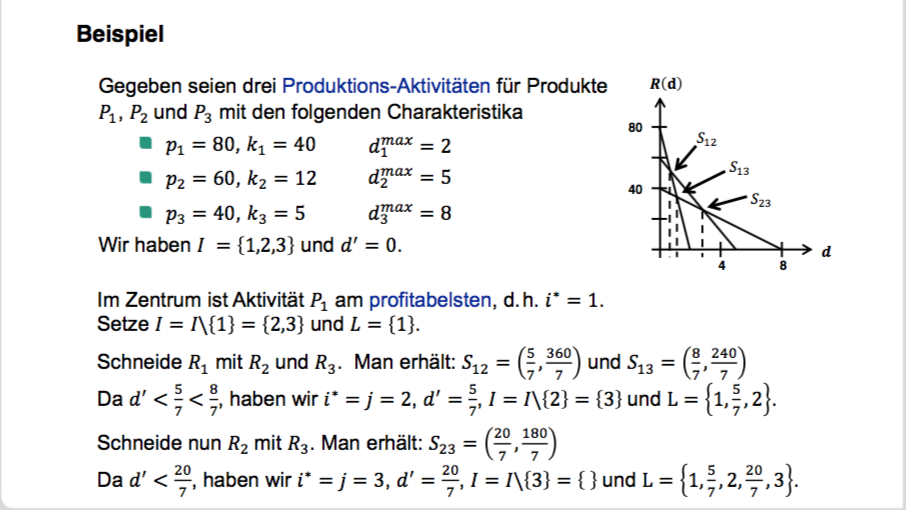
\includegraphics[width=\textwidth]{Images/Theorie_der_Boden_und_Flaechennutzung_BSP(1).png}
          % \caption{}
          % \label{}
        \end{figure}

        \begin{figure}[htbp]
          \centering
          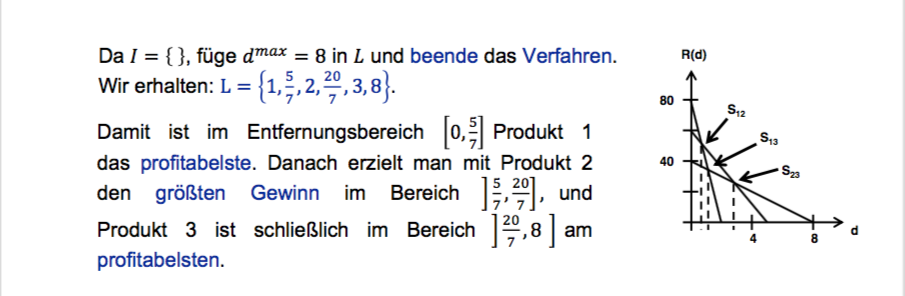
\includegraphics[width=\textwidth]{Images/Theorie_der_Boden_und_Flaechennutzung_BSP(2).png}
          % \caption{}
          % \label{}
        \end{figure}

      \begin{exmp}
        \color{blue}{Aufgabe 3}
      \end{exmp}


    % subsection theorie_der_boden_und_fla_chennutzung (end)

  % section volkswirtschaftliche_standortmodelle (end)

  \section{Deskriptive überbetriebliche Standortmodelle} % (fold)
  \label{sec:deskriptive_berbetriebliche_standortmodelle}
  
    \par Sowohl Prülisten- als auch Rangfolge-Verfahren bestimmen den besten Standort für eine neue Einrichtung basierend auf Standortfaktoren.

    \subsection{Prüflisten-Verfahren} % (fold)
    \label{sub:pr_flisten_verfahren}

      \par Vorgehensweise:

      \begin{itemize}
        \item Zusammenstellung der dem jeweiligen Problem angemessenen Standort-
faktoren. Bei dieser Aufstellung bedarf es großer Umsicht.
        \item Für jeden, der als relevant erachteten Standortfaktoren, ist zu überprüfen und entsprechend zu kennzeichnen, z. B. durch ein Kreuz, an welchem Standort der Faktor küntig am besten erfüllt sein wird.
      \end{itemize}

      \par Bei dieser Vorgehensweise werden einige Standorte mehrere Kennzeichnungen auf sich vereinen und deshalb als besonders günstig erscheinen, während andere möglicherweise leer ausgehen.

      \begin{note}\label{rem:Prüflisten-Verfahren}
        Wähle den Standort mit meisten Kreuze
      \end{note}

      \begin{exmp}
        
      \end{exmp}

      \begin{figure}[htbp]
        \centering
        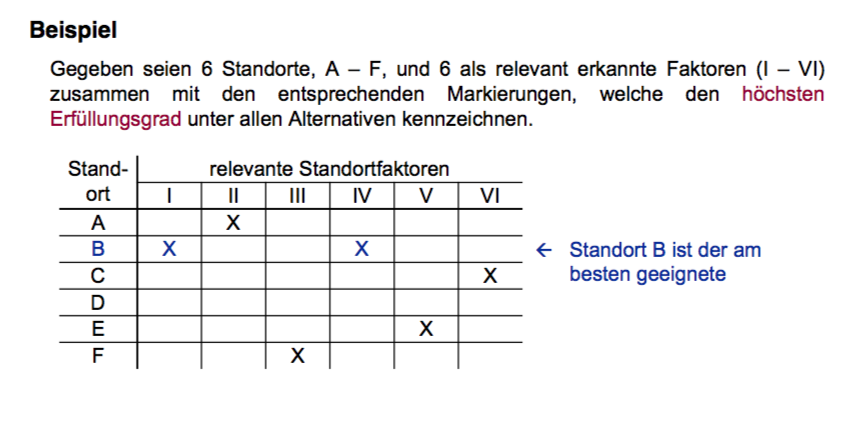
\includegraphics[width=\textwidth]{Images/Prueflisten_Verfahren_BSP.png}
        \caption{Prüflisten-Verfahren Bsp}
        % \label{}
      \end{figure}
    
    % subsection pr_flisten_verfahren (end)

    \subsection{Rangfolge-Verfahren} % (fold)
    \label{sub:rangfolge_verfahren}

      \par Vorgehensweise:

      \begin{itemize}
        \item Zusammenfassung der dem Problem angemessenen Standortfaktoren
        \item Ermittlung einer Gewichtungszahl für jeden Standortfaktoren
        \item Finde die höchste Gesamtwertigkeit
      \end{itemize}

      \begin{exmp}
        
      \end{exmp}

      \begin{figure}[H]
        \centering
        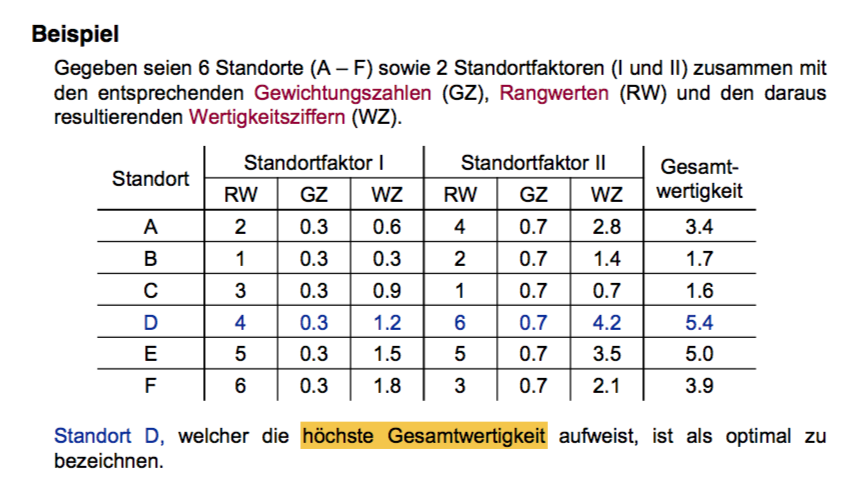
\includegraphics[width=\textwidth]{Images/Rangfolgen_Verfahren_BSP.png}
        \caption{Rangfolge-Verfahren Bsp}
        % \label{fig:label}
      \end{figure}

    
    % subsection rangfolge_verfahren (end)

    \subsection{Vergleich} % (fold)
    \label{sub:vergleich}

      % \begin{table}[]
      %   \centering
      %   \caption{My caption}
      %   \label{my-label}
      %   \begin{tabular}{ccc}\\
      %     & \begin{tabular}[c]{@{}c@{}}1. Durch die Verwendung von Gewichtungszahlen und\\ Rangwerten ist es weitgehend transparent.\\ 2.  Es zerlegt den Entscheidungsprozess in mehrere Einzelschritte, lässt wenig\\ Ermessensspielraum und schöpft den vorhandenen Informationsstand so gut wie\\ möglich aus.\end{tabular} \\
      %     Nachteil & \begin{tabular}[c]{@{}c@{}}1. subjektive Festlegung der relevanten Standortfaktoren problematisch 2. Ankreuztechnik zu kritisieren3. ein gravierender Mangel darin zu sehen, dass es für die einzelnen\\ Standortfaktoren bzw. Kennzeichnungen keine Differenzierung gibt, um unterschiedliche\\ Erfüllungsgrade zu erfassen.\end{tabular} & 1. Subjektivität2. Festlegung der relevanten Standortfaktoren weiterhin problematisch.                                            
        \end{tabular}
        \end{table}
    
    % subsection vergleich (end)

  % section deskriptive_berbetriebliche_standortmodelle (end)

  \section{Standortplanung unter Wettbewerb} % (fold)
  \label{sec:standortplanung_unter_wettbewerb}

    \par Ziel: eine oder mehrere neue Einrichtung so zu platzieren, dass der Marktanteil und Gewinn der eigenen Firma maximiert wird.

    \subsection{Modelle mit vollständiger Zuordnung} % (fold)
    \label{sub:modelle_mit_vollst_ndiger_zuordnung}

      \par Der Bedarf jedes Kunden wird von genau einer Einrichtung vollständig befriedigt. (
      Bei diesen Modellen lässt sich für jeden Kunden eindeutig entscheiden, welche Einrichtung für ihn die Beste oder Attraktivste ist.)

      \begin{defn}
        \textbf{Indifferenzmenge} \\
        die Menge aller Punkte, welche gleichweit von den beiden Standorten $x_A$ und $x_B$ entfernt liegen

        \begin{equation}
          IS_{AB} := \{x \in \mathbb{R} | l_2(x;x_A) = l_2(x; x_B)\}
        \end{equation}
      \end{defn}
      \subsubsection{Voroni-diagramm} % (fold)
         \label{ssub:voroni_diagramm}

          \begin{exmp}
            \color{blue}{Aufgabe 5}
          \end{exmp}
         
         % subsubsection voroni_diagramm (end)   
    % subsection modelle_mit_vollst_ndiger_zuordnung (end)

    \subsection{Modelle mit partieller Aufteilung} % (fold)
    \label{sub:modelle_mit_partieller_aufteilung}

      \par Bei diesen Modellen verteilen die Kunden ihre Nachfrage anteilig auf mehrere Einrichtungen.

      \subsubsection{Gravitions-Modelle (Das Modell von Huff)} % (fold)
      \label{ssub:gravitions_modelle_}

      \begin{defn}
        \textbf{Anziehungskraft der Einrichtung $E$ auf den Kunden $K$}
      \end{defn}
      
      

      \begin{equation}
        A(E, K) = \frac{w_E}{d(K,E) ^ r}
      \end{equation}

      \begin{itemize}
        \item $w_E$: Größe der Einrichtung $E$ an diesem Standort
        \item $d(K, E)$: die Entfernung vom Kunden $K$ zum Standort der Einrichtung $E$
        \item $r$: eine Potenz (Verfallskonstante) für die Entfernung
      \end{itemize}

      \par \textbf{Die Wahrscheinlichkeit $P$}, dass ein Kunde eine Einrichtung an einem bestimmten Standort besucht, berechnet sich nach diesem Modell folgendermaßen:

      \begin{equation}
        P(E, K) = \frac{A(E, K)}{\sum_{\text{alle} \bar{E}}A(\bar{E}, K)}
      \end{equation}

      \begin{defn}
        \textbf{Indifferenzmege zweier Einrichtungen}\\
        die Menge alle Punkte, welche beide Einrichtungen mit derselben Wahrscheinlichkeit aufsuchen.
      \end{defn}

      \par \textbf{Der Anteil der Nachfrage eines Kunden}, welcher auf eine bestimmte Einrichtung entfällt, ergibt sich aus dem Produkt der Gesamtnachfrage des Kunden mit der „Besuchs“-Wahrscheinlichkeit

      \begin{equation}
        D(E, K) = D(K) \cdot P(K, E)
      \end{equation}
      \begin{itemize}
        \item $D(K)$: Gesammtnachfrage des Kunden
      \end{itemize}

      \par \textbf{Gesamtnachfrage einer Einrichtung} = Summe aller Anteile von Kundennachfragen

      \begin{equation}
        D(E) = \sum_{\text{alle } K}D(E, K)
      \end{equation}

      \par \textbf{gesamte Marktanteil der Einrichtung}:

      \begin{equation}
        MS(E) = \frac{D(E)}{\sum_{\text{alle } K}D(K)}
      \end{equation}

      \par Kriterium für Standort einer neuen Einrichtung $\bar{E}$:

      \[ \underset{\bar{E}}{\text{argmax}} \quad \text{MS}(\text{einige Firma}) = \frac{D(\bar{E}) + \sum_{\text{eigene, bereits exist. } E}D(E)}{\sum_{\text{alle } K}{D(K)}}\]

      \textbf{Zusammenfassung}

      \begin{figure}[H]
        \centering
        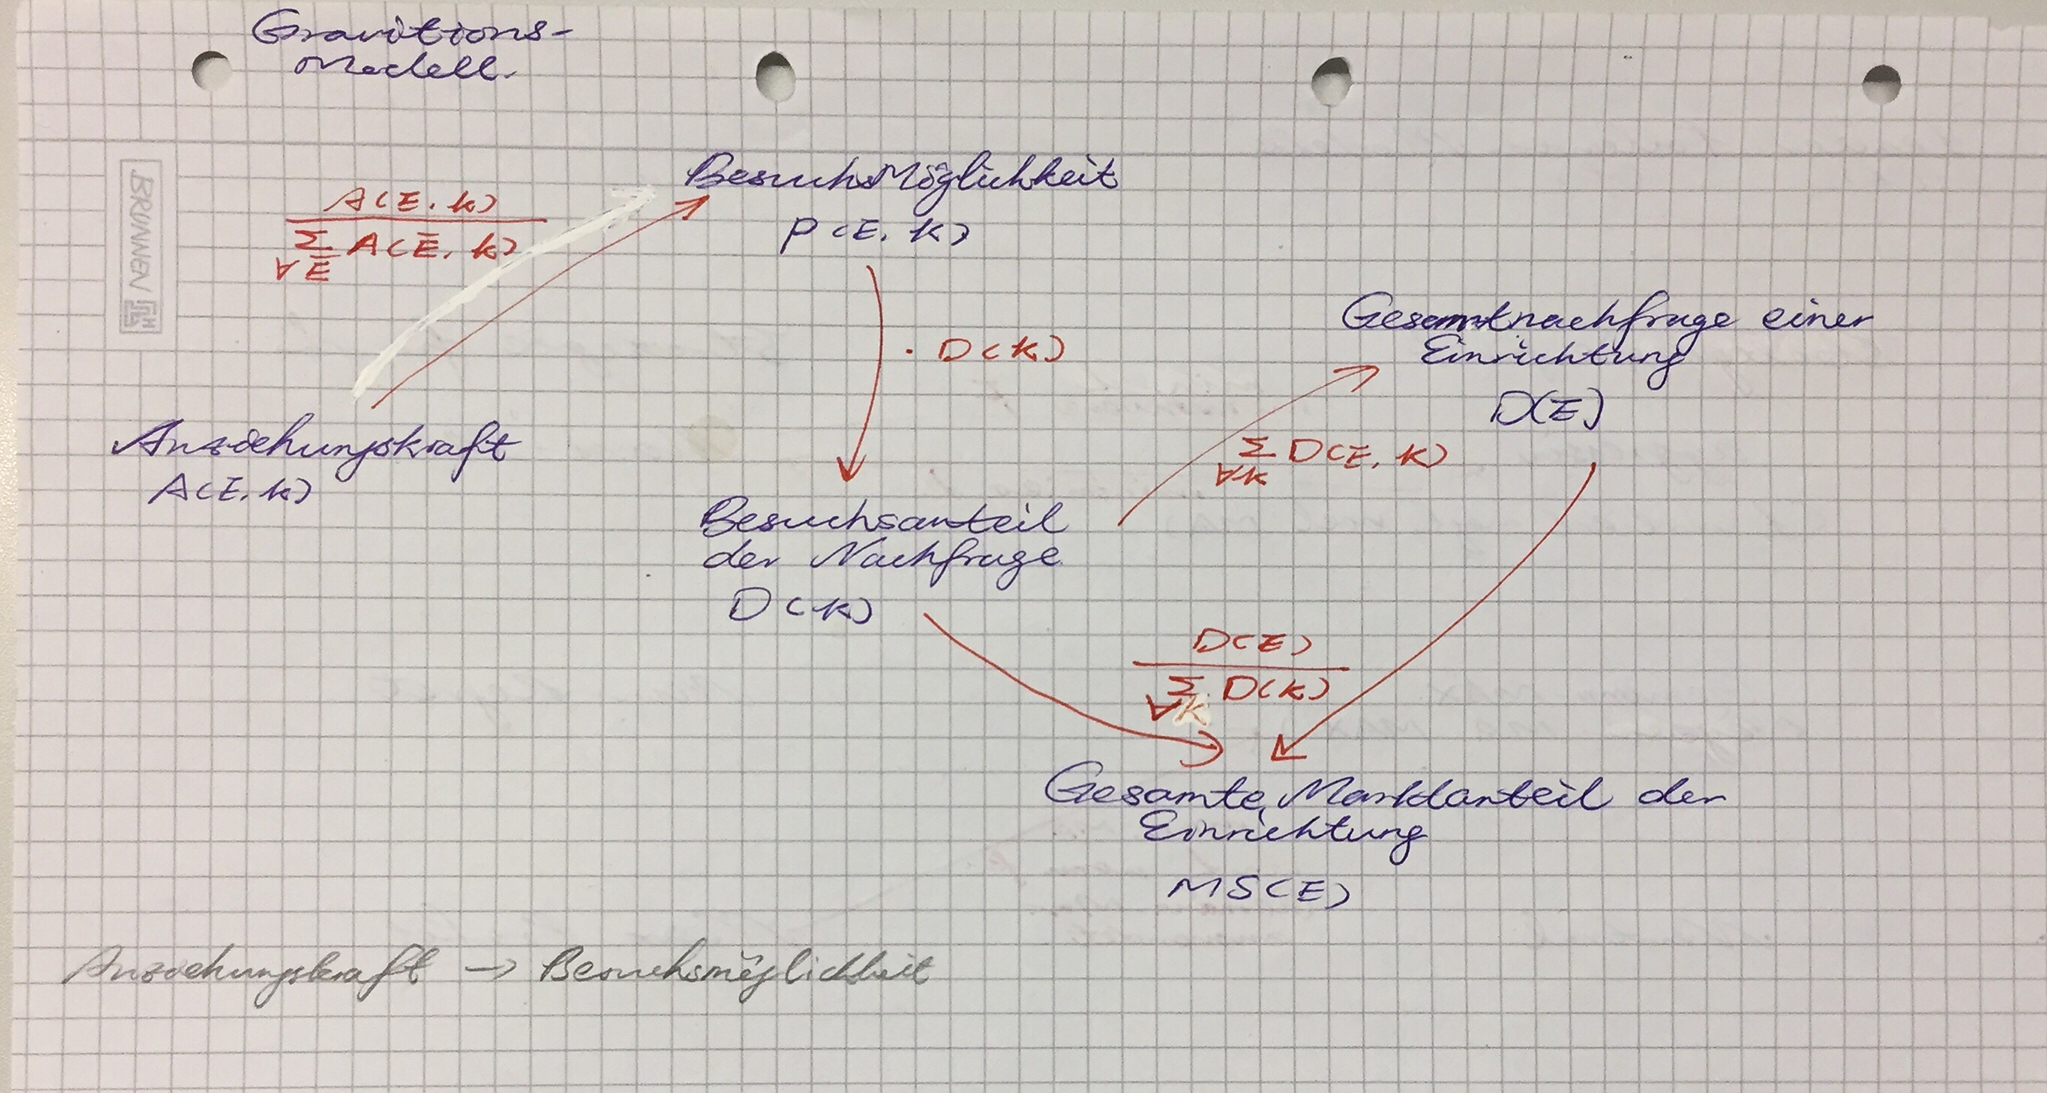
\includegraphics[width=0.95\textwidth]{Images/Gravitionsmodelle.JPG}
        \caption{Gravitionsmodelle}
        \label{fig:Gravitionsmodelle}
      \end{figure}



      \begin{exmp}
         \color{blue}{Aufgabe 4}
       \end{exmp}     
      % subsubsection gravitions_modelle_ (end)

      
    % subsection modelle_mit_partieller_aufteilung (end)

    \subsection{Leader-Follower-Modelle} % (fold)sec
    \label{sub:leader_follower_modelle}

      \subsubsection{Regeln} % (fold)
      \label{ssub:regeln}
        \begin{itemize}
          \item Bei diesen Modellen platzieren zwei Wettbewerber nacheinander neue Einrichtungen in einem (bisher unerschlossenen) Markt.
          \item Dabei wählt zuerst der Leader (Erstplatzierende) $L$ Standorte für all seine neuen Einrichtungen und danach der Follower (Zweitplatzierende) $F$.
          \item Standortwahl von $L$ und $F$ beeinflussen sich gegenseitig.
        \end{itemize}
      % subsubsection regeln (end)

      \subsubsection{Probleme / Herausforderungen} % (fold)
      \label{ssub:probleme_herausforderungen}
        \begin{itemize}
          \item \textbf{Follower $F$}\\
           Braucht sich erst auf eine Platzierungsstrategie festlegen, wenn der Erstplatzierende $L$ seine Standortwahl schon getroffen hat.
          \item \textbf{Leader $L$}\\
          Hat das Problem, dass er die Platzierungsstrategie von $F$ nicht kennt.
        \end{itemize}
      % subsubsection probleme_herausforderungen (end)

      \subsubsection{Typische Stategien für Follower $F$} % (fold)
      \label{ssub:typische_stategien_für_follower}

        \begin{itemize}
          \item \textbf{Aggressiv}\\
          Platziere neue Einrichtungen so, dass $L$ möglichst viel Marktanteil verliert. 

          \item \textbf{Gewinnmaximierend}\\
          Platziere neue Einrichtungen so, dass der eigene Marktanteil maximal wird.

          \item \textbf{Neutral}\\
          Platziere neue Einrichtungen nach anderen Kriterien.
        \end{itemize}
      
      % subsubsection typische_stategien_für_follower (end)

      \subsubsection{Verschiedene Strategien für Leader $L$} % (fold)
      \label{ssub:verschiedene_strategien_für_leader_}
      
        \begin{itemize}
          \item \textbf{Maxi-Min} \\
          $L$ platziert neue Einrichtungen so, dass sein Marktanteil maximal wird, wenn $F$ eine aggressive Strategie anwendet, d. h. $F$ das Ziel hat den Marktanteil von $L$ zu minimieren.

          \begin{framed}
            \textbf{Rechenweg}:
            \begin{enumerate}
              \item Bestimme zu jedem $L$ denjenigen Follower-Standort $\tilde{f}$, der dem Leader den geringsten Gewinn bringt, wenn der Leader bei $l$ platziert.
              \item Berechne den daraus resultierenden Marktanteil des Leaders
              \item Wähle den Standort, für den der Marktanteil des Leaders maximal wird
            \end{enumerate}
          \end{framed}
          
          \item \textbf{Min-Regret (minimales Bedauern)}\\
          $L$ platziert neue Einrichtungen so, dass, egal welche Standortentscheidung $F$ dann trifft, der Zugewinn an Marktanteil für $L$ durch eine mögliche Andersplatzierung seiner Einrichtungen (nachdem $F$ seine Wahl getroffen hat) minimal wird.

          \item \textbf{Max-Profit}\\
          $L$ platziert neue Einrichtungen so, dass ein Marktanteil maximal wird. wenn F ebenfalls eine geweinnmaximierende Strategie anwendet.

          \begin{framed}
            \textbf{Rechenweg}:
            \begin{enumerate}
              \item Bestimme zu jedem $L$ denjenigen Follower-Standort $\tilde{f}$, der dem Follower den größten Gewinn bringt, wenn der Leader bei $l$ platziert.
              \item Berechne den daraus resultierenden Marktanteil des Leaders
              \item Wähle den Standort, für den der Marktanteil des Leaders maximal wird
            \end{enumerate}
          \end{framed}

        \end{itemize}

        \textbf{Zusammenfassung}

        \begin{figure}[htbp]
          \centering
          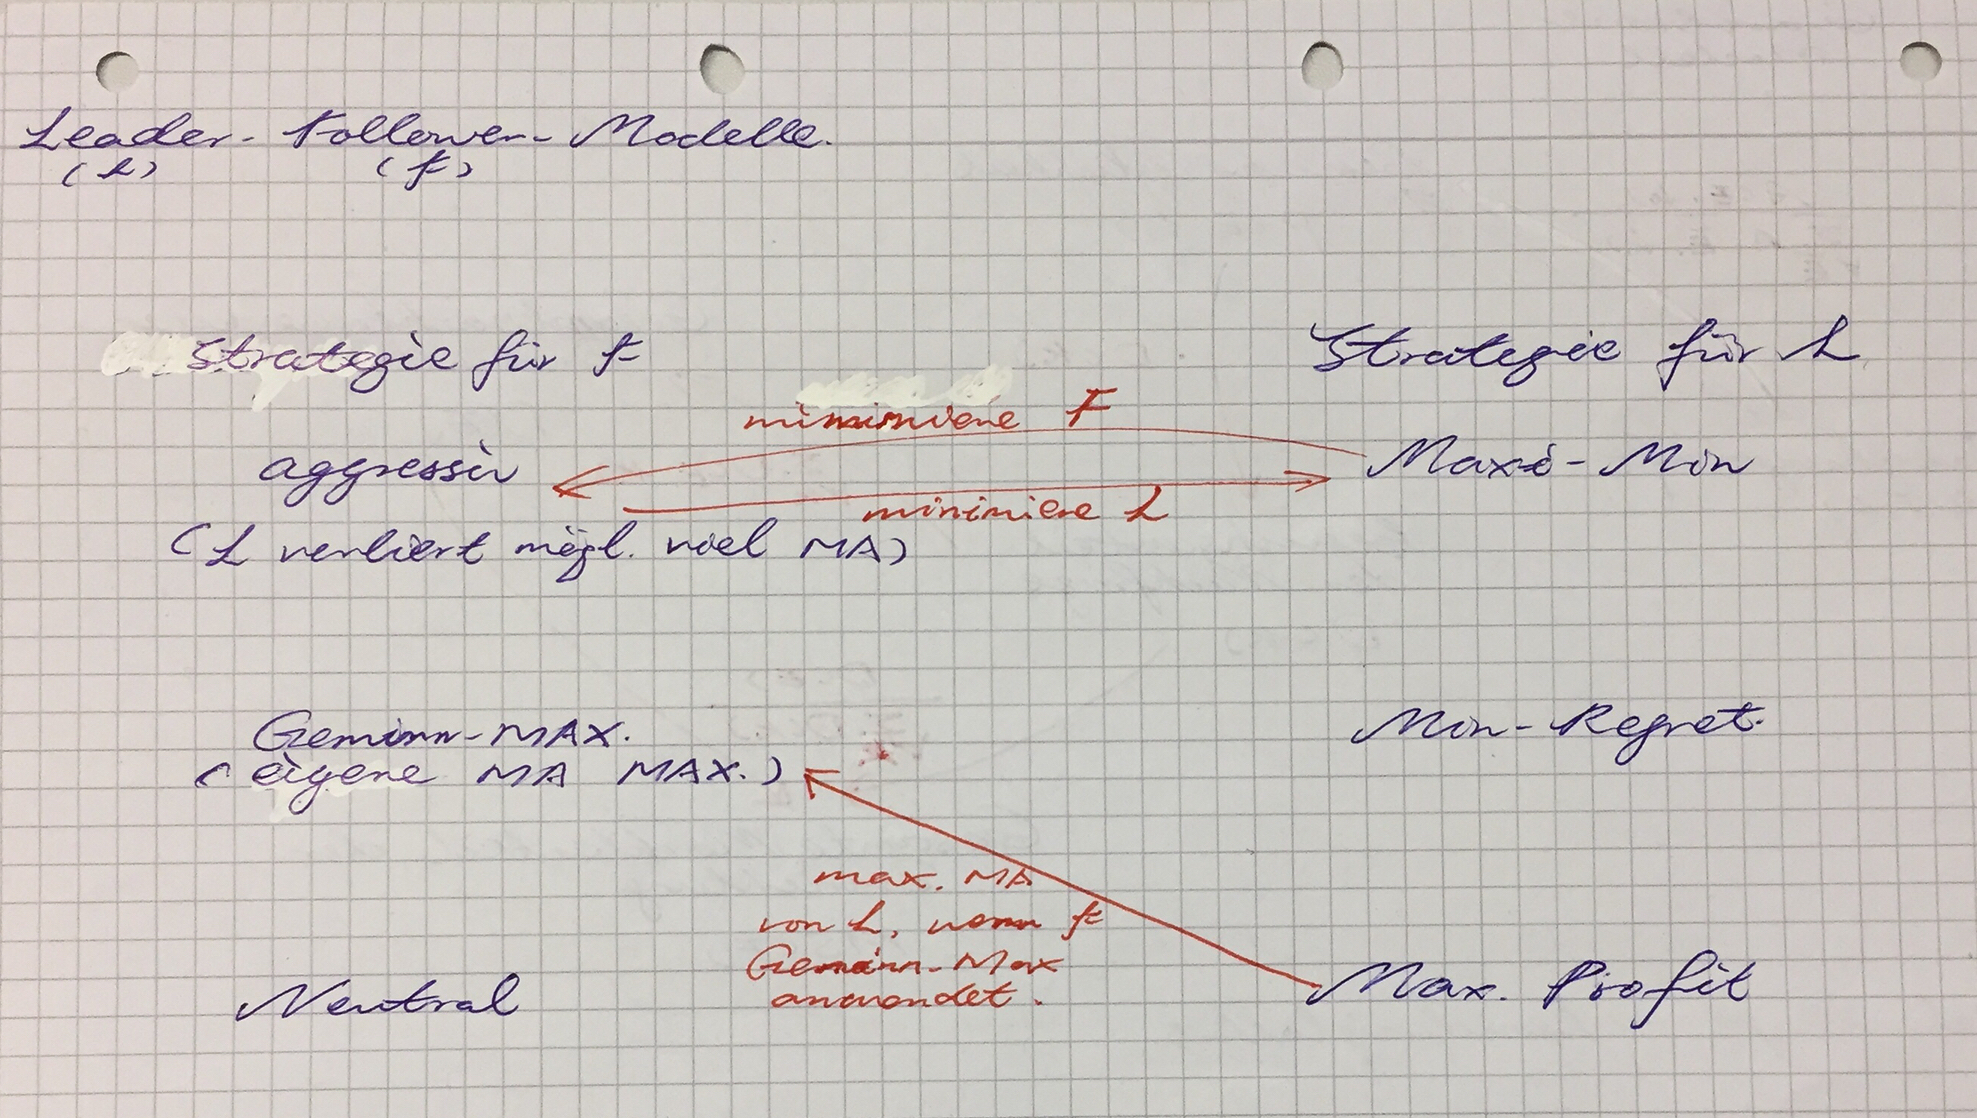
\includegraphics[width=0.95\textwidth]{Images/Leader_Follower_Modelle.JPG}
          \caption{Leader-Follower-Modelle}
          \label{fig:Leader-Follower-Modelle}
        \end{figure}

        \begin{exmp}
         \color{blue}{Aufgabe 6}
       \end{exmp} 
      % subsubsection verschiedene_strategien_für_leader_ (end)
      


    
    % subsection leader_follower_modelle (end)
  
  % section standortplanung_unter_wettbewerb (end)

% chapter volkswirtschaftliche_und_deskriptive_standortmodelle (end)



    
